\documentclass[10pt,conference,compsoc]{IEEEtran}

\usepackage{amsmath}
\usepackage{balance}
\usepackage{booktabs}
\usepackage{graphicx}
\usepackage{microtype}
\usepackage{newtxtext,newtxmath}
\usepackage{url}

\graphicspath{{../../../figures/}}
% Short preprint version for sharing. Build: tectonic talla_grasp_short.tex

\title{Three Ways to Miss a Grasp: A Same-Metric Comparison of Rule-Based, Learned, and Zero-Shot Vision-Language Grasp Prediction}

\author{\IEEEauthorblockN{Anish Talla}
\IEEEauthorblockA{\textit{High School Student}\\
Lightridge High School and Academies of Loudoun\\
Virginia, United States\\
anish.talla99@gmail.com\\
\textit{Preprint, September 2026. Code and data:} \url{https://github.com/anishtalla27/Vision-Based-Grasping}}}

\begin{document}
\maketitle

\begin{abstract}
Accuracy numbers for multimodal models are hard to compare when every
method is tested in its own way. I compared three ways to predict a robotic grasp from an
RGB image under one fixed protocol: a detector-assisted heuristic, a
neural network trained on grasp labels, and a general-purpose
vision-language model (VLM) used zero-shot. All three systems
were tested on the same object-wise split of the Cornell Grasping Dataset and
scored by the same rectangle metric. A fine-tuned ResNet18 passed on 79.7\%
of test images, and a second training round with a stable recipe and three
seeds per architecture put the learned system at 84.0\%. The heuristic
passed on a post-hoc-corrected 57.7\%, up from 40.7\% before the
correction. GPT-4o passed on 12.4\% of 615 calls, five independent runs per image,
with low agreement between runs on identical pixels. Because test images
are repeated views of 35 objects, all intervals come from object-clustered
resampling, which widened every interval and left the order unchanged. The three systems also failed in different ways. The heuristic struggled with
orientation, the ResNet18 usually missed on placement, and GPT-4o failed
both criteria on 59.3\% of calls. Its predicted
center lay outside the convex hull containing all labeled grasp corners on 53.4\%
of parsed calls, compared with 7.0\% and 6.5\% for the other systems. That
pattern suggested the model could see a grasp but not express it as
coordinates. A fourth run tested this directly by showing the same model
label-free candidate grasps drawn on the image and asking it to choose one
by number. On three candidate menus, including one with every mark drawn
the same size, its accuracy stayed at the random floor of the menu, and it
preferred a grasp closing along the object's long axis regardless of mark
size. The model's weak point is choosing the grasp. Writing the
coordinates was never the main problem.
\end{abstract}

\begin{IEEEkeywords}
robotic grasping, vision-language models, GPT-4o, Set-of-Mark prompting,
Cornell Grasping Dataset, clustered bootstrap
\end{IEEEkeywords}

\section{Introduction}

A robot has to make a geometric decision before it can close its gripper:
where the fingers should land, how the gripper should rotate, and how far the
jaws should open. A programmer can write that decision into a set of rules. A
neural network can learn it from labeled examples. A VLM can also be asked for
the answer directly, even if it has never been trained for grasp prediction.
These approaches cost very different amounts to set up, but their reported
accuracies are hard to compare when the input, output, or scoring rule changes
with the method. I treat the comparison as a data analysis problem. The
data, the output format, and the scorer stay fixed, and the one system
that gives different answers on the same input is sampled several times.
The statistics are computed over objects, since objects are the independent
unit here.

I built one system of each kind and kept those parts fixed. Each system saw
the same 123 held-out RGB images, returned the same geometric representation,
and was scored against the same Cornell labels by one implementation of the
standard rectangle test \cite{jiang2011,lenz2015}. I also reconstructed
object identities so that no physical object crossed between training and
test. The statistical analysis resamples whole objects because several test
images are rotated views of the same item.

I queried the VLM 615 times, five separate calls per image, so its
variation on identical input could be measured. I first ask which system predicts the most valid
rectangles, then look at where each system goes wrong, and finally test the most natural explanation
of the VLM's failure with a fourth run that removes its coordinate output. The three systems missed different parts of the
metric. I report those failures with a common taxonomy and a separate check
of whether each predicted center lands near any labeled grasp region.

Current dense grasp detectors already report higher Cornell scores
\cite{kumra2020}. I am not trying to beat them. I want to compare three practical starting
points on one test that does not change with the method.

\section{Related Work}

Jiang \emph{et al.} introduced the Cornell dataset and its rectangle
representation of a grasp \cite{jiang2011}. The rectangle stores the center,
orientation, opening, and jaw depth. Under the usual Cornell test, a
prediction passes when it is within $30^\circ$ of a labeled grasp and its
intersection over union (IoU) is greater than 25\% \cite{lenz2015}. Redmon
and Angelova used a neural network to regress one rectangle and reported
84.9\% object-wise accuracy with RGB-D input \cite{redmon2015}. GR-ConvNet
and other pixel-wise models report higher scores, although they make a dense
prediction instead of regressing one rectangle for the whole image
\cite{kumra2020}.

VLM-based grasping systems usually do not ask the language model for the final
pixel coordinates. Set-of-Mark prompting has the model choose among regions
already marked on an image \cite{yang2024}. VLAD-Grasp has a VLM draw the
grasp, then recovers a pose with depth prediction, segmentation, and
point-cloud alignment \cite{kulshrestha2025}. System C tests a smaller
pipeline: show GPT-4o the image and ask it to return the coordinates itself.
So its score says something about that way of asking. It does not set a
limit on what VLM-based grasping can do.

\section{Experimental Design}

\subsection{Dataset, Split, and Metric}

Cornell contains 885 RGB-D images of household objects, with several positive
grasp rectangles on most images. I used only RGB. Two images were dropped
because their object boundaries could not be resolved, leaving 883.

Cornell does not include object IDs, so I reconstructed them from the frame
sequence. The procedure segmented the object from the photography platform
and compared consecutive masks with color and area descriptors that tolerate
rotation. Ambiguous boundaries were reviewed manually. The two possible mistakes are not equally bad, so I set the thresholds
unevenly. If two
objects are merged, the combined group still stays in one split. If one
object is split in two, its images can leak into both training and test.

An automated first pass assigned a decision and confidence to each ambiguous
boundary. In a blind 30-boundary audit, its calls agreed with my labels on
86.7\% of confident cases and 40.0\% of uncertain ones. I then decided every
uncertain call and every high-risk ``different object'' call. Table
\ref{tab:split} shows the final seed-42 split. A second check confirmed that
no object appears in more than one partition.

\begin{table}[t]
\caption{Object-wise Cornell split.}
\label{tab:split}
\centering
\begin{tabular}{lrr}
\toprule
Partition & Objects & Images \\
\midrule
Train & 164 & 620 \\
Validation & 35 & 140 \\
Test & 35 & 123 \\
\midrule
Total & 234 & 883 \\
\bottomrule
\end{tabular}
\end{table}

I scored each prediction against every positive rectangle on its image. A
match to any one of them counts as correct. Before using the evaluator at
scale, I checked hand-computed cases, rectangle round trips, and an independent
rasterized IoU calculation. All predictions were converted back to the native
$640\times480$ coordinate frame for the final comparison.

\subsection{System A: Detector-Assisted Heuristic}

System A starts with a COCO-pretrained Faster R-CNN using a
ResNet50-FPN-v2 backbone \cite{ren2015}. A fixed lookup table maps the detected
category to a center, upper, or end grasp. I calibrated the global opening and
jaw-size constants on training labels only. The COCO vocabulary misses most
Cornell objects, so a platform-segmentation fallback supplies a box when the
detector cannot. The rule closes the gripper across the box's narrow
dimension. It can output only $0^\circ$ or $90^\circ$.

The first test run scored 40.7\%. Its rendered predictions exposed a defect:
some accepted detections covered background clutter instead of the object on
the platform. I added a guard requiring the detection to contain the
segmented object's centroid and recalibrated the global constants on training
data. The score rose to 57.7\%. Test output prompted that change, so 57.7\%
is post-hoc and 40.7\% remains the clean pre-correction result.

\subsection{System B: Learned Predictor}

System B replaces ResNet18's ImageNet classifier \cite{he2016} with separate
heads for center, orientation, and size. The orientation head predicts
$(\cos 2\theta,\sin 2\theta)$. Doubling the angle handles the fact that a
parallel-jaw grasp is unchanged by a $180^\circ$ rotation. For images with
several labels, I compute the loss against every rectangle and backpropagate
only the best match. Averaging all valid labels could put the target between
two good grasps, where neither one actually exists.

I trained a custom CNN, ResNet18, and ResNet34 on the 620 training images.
Affine augmentation moved the rectangle corners with the pixels. Architecture,
checkpoint, size-loss weight, and the custom CNN's learning rate were chosen
on validation data. ResNet18 had the best validation accuracy at 83.6\%, so I
froze that model before opening the test results.

That first round trained each architecture once, at one seed, with a
constant learning rate, and kept the best of roughly a hundred noisy
validation epochs. A second round kept the model, loss, data, and split and
changed only the recipe: cosine learning-rate decay over a fixed 100 epochs,
an exponential moving average of the weights, three seeds per architecture,
and no checkpoint selection, with the final averaged weights reported.
Test-time augmentation over eight dihedral views, combined by taking the
medoid rectangle, was adopted only because it raised mean validation
accuracy. Four selection rules were written down before the test split was
opened a second time, and every configuration that touched test is reported.

\subsection{System C: Zero-Shot VLM}

System C sends the native RGB image to GPT-4o through OpenRouter
\cite{openai2024}. It uses no grasp-specific training. The prompt asks for two
fingertip coordinates and a jaw width in JSON, which together define the
rectangle. I developed the prompt on 30 training images and froze it before
test.

Each test image was sent in five independent, single-turn calls at the
provider's default temperature. I retried transport failures, but not replies
that arrived and failed to parse. Retrying those would quietly turn a
single-call baseline into a best-of-several system. Of 615 calls, 614 parsed.
The primary score pools the five exchangeable runs to estimate one-call
accuracy. Best-of-five is only a ceiling: it requires five calls and an oracle
that knows when one of them is right.

\subsection{System D: Marked-Candidate Selection}

If GPT-4o can see where to grasp but cannot express it as coordinates,
removing the coordinate output should recover its choice. System D shows the
same model the same test images with candidate grasps drawn on a zoomed crop
and asks for the number of the one it would use. Candidates come only from
the platform-segmentation mask: principal-component analysis gives the
centroid, long axis, and extent, and candidates are positions along the long
axis crossed with four jaw-travel directions 45$^\circ$ apart, so every grasp
angle is within the metric's tolerance of some candidate. Opening and jaw
width use System A's train-calibrated constants. Numbering is re-shuffled on
every call. Because the menu is fixed before the model sees it, each run
carries its own floor (expected accuracy of a uniformly random choice) and
ceiling (whether any candidate passes).

Three menus were run, each on the full test split with five repeats. The
first had twelve marks at three positions. The second had four marks at
the centroid only, drawn at real size. The third had the same four marks
drawn at one uniform length, and its prompt said that length is not to
scale. The last two exist because on thin
objects the correct marks are the smallest on the image, so a preference for
large marks would mimic a preference for the long-axis grasp. The prompt was
developed on 30 training images for parse rate and glyph reading only, and
each menu's test run was called once under its own sentinel.

\subsection{Statistical and Failure Analysis}

The 123 test images are repeated views of 35 unseen objects, not 123
independent samples. I formed the 95\% confidence intervals from 20,000
object-clustered bootstrap resamples. Every view of an object, along with all
five VLM calls, moves together. Paired differences use the same resamples and
20,000 object-level label-swap permutations.

The failure analysis gives each attempt one label: correct, angle only,
overlap only, both criteria, or no prediction. I also checked whether the
predicted center falls inside the convex hull of all labeled grasp corners on
the image. This is a loose spatial check, not a claim that the grasp would
work on hardware. A center outside that hull falls beyond the area spanned by
the annotated grasp corners.

\section{Results}

\subsection{Overall Accuracy}

ResNet18 passed 98 of 123 images (79.7\%). The corrected heuristic passed 71
(57.7\%), and GPT-4o passed 76 of 615 calls (12.4\%). Its five runs ranged
from 9.8\% to 14.6\%. At least one GPT-4o call passed on 43 of the 123 images,
which gives a best-of-five ceiling of 35.0\%. Table~\ref{tab:accuracy} includes
the object-clustered intervals.

\begin{table}[t]
\caption{Accuracy with object-clustered 95\% confidence intervals.}
\label{tab:accuracy}
\centering
\begin{tabular}{lrr}
\toprule
System & Accuracy & 95\% CI \\
\midrule
A: heuristic, corrected & 57.7\% & [46.2, 68.2] \\
B: ResNet18, round 1 & 79.7\% & [70.8, 87.1] \\
B: ResNet34, round 2, 3 seeds & \textbf{84.0\%} & [73.9, 92.1] \\
C: GPT-4o, one call & 12.4\% & [8.0, 17.4] \\
C: best of five & 35.0\% & [24.6, 45.5] \\
\bottomrule
\end{tabular}
\end{table}

ResNet18 led the corrected heuristic by 22.0 points. The bootstrap interval
for that difference was [9.7, 35.1], with permutation $p=0.0031$. The
corrected heuristic led GPT-4o's best-of-five ceiling by 22.8 points [9.2,
35.6], $p=0.0060$, and its expected one-call score by 45.4 points [33.8,
55.6], $p<0.0001$. Giving each object equal weight produced 51.3\%, 75.4\%,
and 10.5\% for A, B, and one-call C. That calculation changed the size of the
gaps but not their order.

The second training round chose ResNet34 on mean final-weight validation
accuracy (81.4\% against 81.2\% for ResNet18) and used augmentation. Its
three seeds scored 84.6, 83.7, and 83.7\% on test, a mean of 84.0\% with
interval [73.9, 92.1]. ResNet18 under the same recipe averaged 82.6\%.
Re-running the first-round recipe at two new seeds gave 82.9\% and 80.5\%,
so 79.7\% was a low-side single draw, and the first round's nine-point gap
between ResNet18 and ResNet34 was run-to-run noise. Round 2 leads A by 26.3
points [14.8, 38.3], $p=0.0002$. Its 4.3 point lead over round 1 does not
exclude zero.

\subsection{Failure Patterns}

The error counts in Table~\ref{tab:taxonomy} tell the systems apart better
than the accuracy numbers do. Thirteen of A's 52 failures had enough overlap and missed
only the angle test, which fits a system limited to two orientations. B had
four angle-only failures. Fifteen of its 25 misses failed only on overlap, so
placement was the larger remaining problem. C failed both tests on 365 of 615
calls (59.3\%).

\begin{table}[t]
\caption{Shared failure taxonomy. Percentages use all attempts.}
\label{tab:taxonomy}
\centering
\footnotesize
\begin{tabular}{lrrr}
\toprule
Outcome & A ($n=123$) & B ($n=123$) & C ($n=615$) \\
\midrule
Correct & 71 (57.7) & 98 (79.7) & 76 (12.4) \\
Angle only & 13 (10.6) & 4 (3.3) & 85 (13.8) \\
Overlap only & 18 (14.6) & 15 (12.2) & 88 (14.3) \\
Both & 13 (10.6) & 6 (4.9) & 365 (59.3) \\
No prediction & 8 (6.5) & 0 (0.0) & 1 (0.2) \\
\bottomrule
\end{tabular}
\end{table}

The center-hull check shows where C's failures begin. A landed outside the
labeled grasp hull on 8 of 115 predictions (7.0\%), and B did so on 8 of 123
(6.5\%). C did so on 328 of 614 parsed calls (53.4\%). Figure
\ref{fig:comparison} shows the shared coordinate frame on one image. This is
not an even contest by itself: A starts from a detected or segmented object,
and B was trained on Cornell. C can place its coordinates anywhere. I use
this check only to see where C's failures start. The three rates should
not be read as measuring the same skill.

\begin{figure}[t]
\centering
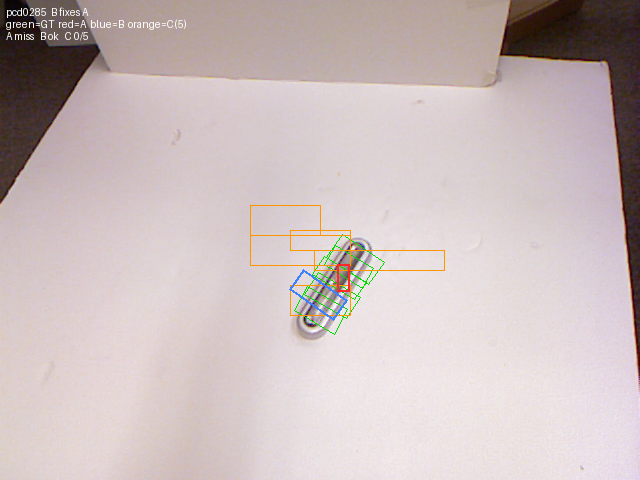
\includegraphics[width=\columnwidth]{compare_0285.png}
\caption{One test image under the shared coordinate system. Labeled grasps
are green, System A red, System B blue, and System C's five repeats orange.}
\label{fig:comparison}
\end{figure}

The five GPT-4o calls also disagreed with one another. Mean pairwise rectangle
agreement was 22.0\%, and mean pairwise IoU was 0.13. All five calls failed on
80 of 123 images. All five passed on one image. The remaining 42 images were
unstable: identical pixels sometimes produced a passing grasp and sometimes
did not.

\subsection{System D}

Table~\ref{tab:menus} gives the three menus. On none of them does the
model's one-call accuracy differ from a random choice among the same
candidates (paired object-clustered differences $-1.4$ [$-6.6$, $+4.0$],
$+1.9$ [$-2.2$, $+6.3$], and $-2.3$ [$-6.3$, $+1.7$]), while the ceilings
are 79.7\% and 65.9\%. Its choices are not random, though. On the full
menu it chose the candidate whose jaws travel along the object's long axis
near one end in 61\% of calls, a grasp type that passes 17\% of the time,
with reasoning such as ``grips the narrow top edge near the center of
mass''. With four marks at the centroid drawn at one uniform size, it still
chose the long-axis direction in 45\% of calls against a 25\% chance rate,
and the short-axis candidate, which passes on 55\% of images, in 17\%.
Stated confidence was ``high'' on 556 of 560 full-menu calls, 21\% of them
correct. Every reply parsed. The candidate at the centroid closing across
the short axis, with no model at all, scored 55.3\% [41.8, 68.0], level
with System A.

\begin{table}[t]
\caption{System D on three candidate menus, same model and test images,
five repeats each. ``Long axis'' is the share of calls choosing the
orientation whose jaws travel along the object's long axis; chance is 25\%
on the four-mark menus.}
\label{tab:menus}
\centering
\footnotesize
\begin{tabular}{lrrrrr}
\toprule
Menu & Marks & Acc. & Floor & Ceil. & Long axis \\
\midrule
Full, 3 positions & 12 & 18.7 & 20.1 & 79.7 & 70\% \\
Centroid, real & 4 & 26.5 & 24.6 & 65.9 & 41\% \\
Centroid, uniform & 4 & 22.3 & 24.6 & 65.9 & 45\% \\
\bottomrule
\end{tabular}
\end{table}

\section{Discussion and Limitations}

On this setup, asking GPT-4o for raw coordinates worked poorly. I am not
claiming that about VLM grasping methods in general. Set-of-Mark and VLAD-Grasp
use a VLM without making it emit the final coordinates, and both add machinery
that System C does not have \cite{yang2024,kulshrestha2025}.

On a sample of C's failures, I read rationales that named a plausible part of
the object while the coordinates landed elsewhere, which together with the
53.4\% center-hull rate suggested a coordinate-binding hypothesis: the model
recognizes a useful region in words and loses it while mapping the answer
into pixels. System D tested that hypothesis and it failed. Taking the
coordinates away and offering a menu with a 79.7\% ceiling did not recover
the choice, and the preference for closing along the long axis survived
menus with no end-straddling candidates and with every mark the same size.
From a top-down photograph, two fingertip pads straddling the end of an
elongated object do look like they pinch a narrow part. In three dimensions
the second finger lands on top of the object. The failure is better
described as grasp reasoning from a single 2-D view than as text failing to
bind to coordinates.

The experiment has several limits. It uses one object-wise split of a small
benchmark, RGB without depth, and no robot trials. Cornell's annotations are
not exhaustive, so a rectangle that fails the metric might still work on a
real object. System B also received more development effort: three
architectures, validation-based tuning, and a second training round,
compared with one frozen prompt for C and D. The test split was opened
twice for System B, once per round, under rules fixed beforehand, but two
openings are still two. System D used one glyph style and one candidate
generator. An early formatting check on about 550 grasp rectangles probably
included a few images that later entered test, although no parameter or rule
came from that check. Test inspection also prompted System A's correction.
Its 40.7\% score is the clean pre-correction result, and comparisons
using 57.7\% are post-hoc. To confirm these results I would need a fresh split or a second dataset.

\section{Conclusion}

ResNet18 scored highest at 79.7\%, and 84.0\% averaged over three seeds
under a stable recipe. The corrected heuristic reached 57.7\%, and GPT-4o
reached 12.4\% per call. Where each one goes wrong matters as much as that
ranking. The heuristic often found the object but could not represent
its angle. ResNet18 usually got the angle and missed the placement. GPT-4o
often failed before either distinction mattered because its rectangle was not
near a labeled grasp region.

Given marked candidate grasps instead of a coordinate output, the same model
chose no better than chance on three menus and kept preferring an end pinch
along the object's long axis even when every mark was drawn the same size.
The problem is the grasp choice, not its expression. A label-free rule that
closes across the segmented object's short axis matches the detector-based
heuristic while handling diagonal objects, and is the cheapest system here
to build. What remains untested is whether depth input, or a model with a
stronger three-dimensional prior, changes the choice.

\section*{Acknowledgment}

OpenAI Codex helped restructure, shorten, and edit an earlier conference
version of this manuscript from my existing report, code, and verified
results. Anthropic Claude Code helped with code development, made the
first-pass calls on ambiguous object boundaries, implemented the second
training round and System D under my design, and helped edit this
version. I designed the study, made the research decisions, ran and checked
the experiments, verified the citations and numerical claims, and approved
the final text. GPT-4o was evaluated separately as System C in Section III-C.

\balance
\begin{thebibliography}{00}

\bibitem{jiang2011}
Y. Jiang, S. Moseson, and A. Saxena, ``Efficient grasping from RGBD images:
Learning using a new rectangle representation,'' in \emph{Proc. IEEE Int.
Conf. Robot. Autom. (ICRA)}, 2011, pp. 3304--3311.

\bibitem{lenz2015}
I. Lenz, H. Lee, and A. Saxena, ``Deep learning for detecting robotic
grasps,'' \emph{Int. J. Robot. Res.}, vol. 34, nos. 4--5, pp. 705--724, 2015.

\bibitem{redmon2015}
J. Redmon and A. Angelova, ``Real-time grasp detection using convolutional
neural networks,'' in \emph{Proc. IEEE Int. Conf. Robot. Autom. (ICRA)},
2015, pp. 1316--1322.

\bibitem{kumra2020}
S. Kumra, S. Joshi, and F. Sahin, ``Antipodal robotic grasping using
generative residual convolutional neural network,'' in \emph{Proc. IEEE/RSJ
Int. Conf. Intell. Robots Syst. (IROS)}, 2020, pp. 9626--9633.

\bibitem{yang2024}
J. Yang \emph{et al.}, ``Set-of-Mark prompting unleashes extraordinary
visual grounding in GPT-4V,'' \emph{arXiv:2310.11441}, 2023.

\bibitem{kulshrestha2025}
M. Kulshrestha \emph{et al.}, ``VLAD-Grasp: Zero-shot grasp detection via
vision-language models,'' \emph{arXiv:2511.05791}, 2025.

\bibitem{ren2015}
S. Ren, K. He, R. Girshick, and J. Sun, ``Faster R-CNN: Towards real-time
object detection with region proposal networks,'' in \emph{Adv. Neural Inf.
Process. Syst.}, vol. 28, 2015.

\bibitem{he2016}
K. He, X. Zhang, S. Ren, and J. Sun, ``Deep residual learning for image
recognition,'' in \emph{Proc. IEEE Conf. Comput. Vis. Pattern Recognit.
(CVPR)}, 2016, pp. 770--778.

\bibitem{openai2024}
OpenAI, ``GPT-4o system card,'' \emph{arXiv:2410.21276}, 2024.

\end{thebibliography}

\end{document}
